\documentclass[../../main.tex]{subfiles}

\begin{document}
\section{No Power-Law in Hidden Markov Models}
    When modelling \emph{natural language}, we generate the next token(s) based on the previous tokens (and hence not based on future tokens; we generate text from left to right). Thus, when disregarding the future tokens, i.e. when marginalizing over them, we can determine the Markov blanket of the current token, i.e. determine the minimal set of tokens that infuluence the current one.

    Naturally, we can think of natural language modelling as \emph{Bayesian networks} over the characters in the text. Because we generate text from left to right, we naturally assume all arrows to go from previous tokens to future tokens (because this is also the modus operandi for token generation). For example, Markov chains up to character position $t$ have the following simple representation:

    \begin{figure}[h]
        \center
        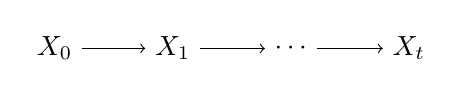
\begin{tikzpicture}[node distance=1.5cm, auto]
        \node (X0) {$X_0$};
        \node (X1) [right of=X0] {$X_1$};
        \node (dots) [right of=X1] {$\cdots$};
        \node (Xt) [right of=dots] {$X_t$};

        \draw[->] (X0) -- (X1);
        \draw[->] (X1) -- (dots);
        \draw[->] (dots) -- (Xt);
        \end{tikzpicture}
        \caption{Bayesian network of Markov chains. All arrows go from previous tokens to future tokens.}
        \label{fig:bayesian_network_markov_chain}
    \end{figure}

    But really, in Markov chains $P(X_{t + 1} = a \mid X_t = b)$ is independent of $t$ and hence is constant over time. So really, all the arrows in figure~\ref{fig:bayesian_network_markov_chain} represent the same transition, this is very important to note.

    From a modelling perspective, it is very reasonable to reuse the same transitions over time, as we cannot have infinitely many "hard-coded" transitions (but we can use different models whith implicitely infitite transitions). Furthermore, for the same \emph{mode of transition}, which we define as the "arrow structure" in the Bayesian network (in figure~\ref{fig:bayesian_network_markov_chain} the mode of transition would be from the current token to the next), it seems reasonable to assume invariance in time for a single constant mode of transition based on the characteristics of natural language.

    Now, the question is, can we achieve power law decay with only one constant (hard-coded) mode of transition? Well, for Markov chains it did not work, so maybe we just have to augment the context window and create new modes of transition.

    This is an interesting approach, which we will investigate on. Since we already established interesting results for Markov chains, we would like to reduce any constant mode of transition to a Markov chain. But how do we do this for a larger context window, where we have many random variables influencing the current one?
    
    The idea is to employ a hidden variable $Y \in \Sigma ^s$, where $\Sigma$ is the alphabet, and $s$ is the size of the context window, which we define as the length of the longest arrow in the mode of transition (for Markov chains $s = 1$). Clearly, $Y$ captures the entire \emph{state} at time $t$ of our model, and we can model the transitions $Y_t \to Y_{t + 1}$ as simple Markov chain transitions (and hence independent of time). And, of course, once we know $Y_t$, we also know $X_t$ (which of course can be modelled with Markov chain transitions as well). Thus, we have the following Bayesian network:

    \begin{figure}[h]
        \center
        \begin{tikzpicture}[node distance=1.5cm and 1.5cm, auto]

        % Top row (Y)
        \node (Y0) {$Y_0$};
        \node (Y1) [right of=Y0] {$Y_1$};
        \node (Ydots) [right of=Y1] {$\cdots$};
        \node (Yt) [right of=Ydots] {$Y_t$};

        % Bottom row (X)
        \node (X0) [below of=Y0] {$X_0$};
        \node (X1) [right of=X0] {$X_1$};
        \node (Xdots) [right of=X1] {$\cdots$};
        \node (Xt) [right of=Xdots] {$X_t$};

        % Horizontal arrows (Y row)
        \draw[->] (Y0) -- (Y1);
        \draw[->] (Y1) -- (Ydots);
        \draw[->] (Ydots) -- (Yt);

        % Vertical arrows
        \draw[->] (Y0) -- (X0);
        \draw[->] (Y1) -- (X1);
        \draw[->] (Yt) -- (Xt);

        \end{tikzpicture}
        \caption{Bayesian network of a hidden Markov model.}
        \label{fig:bayesian_network_hidden_markov}
    \end{figure}

    These models are known as \emph{hidden Markov models}. Unfortunately, there is no free lunch, as we see in the following theorem:

    \begin{theorem}[No Hidden Markov Model with Power-Law decay]
        There is no hidden Markov model $(\bm{M_Y}, \bm{M_X})$ with $I(X_{t_0}, X_{t_0 + \tau}) \in \mathcal{O}(\tau^{-\alpha})$ and $I(X_{t_0}, X_{t_0 + \tau}) \in \Omega (\tau^{-\beta})$ for some $\alpha, \beta \in \mathbb{R}_{>0}$.
    \end{theorem}
    \vspace{-2.5em}
    \begin{proof}
        Set $t \coloneqq t_0$. First, note that $P(X_{t + \tau} = b \mid Y_t = c) = (\bm{M_X} \bm{M_Y}^\tau)_{bc}$. Furthermore,
        \begin{align*}
            P(Y_t = c \mid X_t = a) &= \dfrac{P(Y_t = c, X_t = a)}{P(X_t = a)} \\
            &= \dfrac{P(X_t = a \mid Y_t = c) P(Y_t = c)}{P(X_t = a)} \\
            &= (\bm{M_X})_{ac} \dfrac{P(Y_t = c)}{P(X_t = a)} \quad .
        \end{align*}
        We are interested in $P(X_{t + \tau} = b \mid X_t = a)$. Based on our observations, we have
        \begin{align*}
            P(X_{t + \tau} = b \mid X_t = a) &= \sum_{c \in S_Y} P(Y_t = c \mid X_t = a) P(X_{t + \tau} = b \mid Y_t = c) \\
            &= \sum_{c \in S_Y} (\bm{M_X})_{ac} \dfrac{P(Y_t = c)}{P(X_t = a)} (\bm{M_X} \bm{M_Y}^\tau)_{bc} \\
            &= \dfrac{1}{P(X_t = a)} \sum_{c \in S_Y} (\bm{M_X})_{ac} P(Y_t = c) (\bm{M_X} \bm{M_Y}^\tau)_{bc} \\
            &= \dfrac{1}{P(X_t = a)} \sum_{c \in S_Y} (\bm{M_X})_{ac} P(Y_t = c) \sum_{d \in S_Y} (\bm{M_X})_{bd} (\bm{M_Y}^\tau)_{dc} \quad . \\
        \end{align*}
        For the case that $\bm{M_Y}^\tau$ converges to $\bm{M_{\mu_Y}}$, it must do so with exponential decay. So we get:
        \begin{align*}
            &= \dfrac{1}{P(X_t = a)} \sum_{c \in S_Y} (\bm{M_X})_{ac} P(Y_t = c) \sum_{d \in S_Y} (\bm{M_X})_{bd} ((\bm{\mu_Y})_{d} \pm \mathcal{O}(|\lambda_2^+|^\tau)) \\
            &= \dfrac{1}{P(X_t = a)} \sum_{c \in S_Y} (\bm{M_X})_{ac} P(Y_t = c) \left[ (\bm{M_X}\bm{\mu_Y})_{b} \pm \mathcal{O}(|\lambda_2^+|^\tau) \right] \\
            &= \dfrac{1}{P(X_t = a)} \sum_{c \in S_Y} \left[ (\bm{M_X})_{ac} P(Y_t = c) (\bm{M_X}\bm{\mu_Y})_{b} \pm \mathcal{O}(|\lambda_2^+|^\tau) \right] \\
            &= \left[ \dfrac{1}{P(X_t = a)} \sum_{c \in S_Y} (\bm{M_X})_{ac} P(Y_t = c) (\bm{M_X}\bm{\mu_Y})_{b} \right] \pm \mathcal{O}(|\lambda_2^+|^\tau) \\
            &= \left[ \dfrac{(\bm{M_X}\bm{\mu_Y})_{b}}{P(X_t = a)} \sum_{c \in S_Y} (\bm{M_X})_{ac} P(Y_t = c) \right] \pm \mathcal{O}(|\lambda_2^+|^\tau) \\
            &= \left[ \dfrac{(\bm{M_X}\bm{\mu_Y})_{b}}{P(X_t = a)} P(X_t = a) \right] \pm \mathcal{O}(|\lambda_2^+|^\tau) \\
            &= (\bm{M_X}\bm{\mu_Y})_{b} \pm \mathcal{O}(|\lambda_2^+|^\tau) \quad . \\
        \end{align*}
        Thus, we get:
        \begin{align*}
            I_R(X_t, X_{t + \tau}) + 1 &= \sum_{(a,b) \in {S_X}^2} \dfrac{P(X_t = a)}{P(X_{t + \tau} = b)} P(X_{t + \tau} = b \mid X_t = a)^2 \\
            &= \sum_{(a,b) \in {S_X}^2} \dfrac{P(X_t = a)}{P(X_{t + \tau} = b)} \left[ (\bm{M_X}\bm{\mu_Y})_{b} \pm \mathcal{O}(|\lambda_2^+|^\tau) \right] ^2 \\
            &= \sum_{(a,b) \in {S_X}^2} \dfrac{P(X_t = a)}{P(X_{t + \tau} = b)} \left[ (\bm{M_X}\bm{\mu_Y})_{b}^2 \pm \mathcal{O}(|\lambda_2^+|^\tau) \right] \\
            &= \left[ \sum_{(a,b) \in {S_X}^2} \dfrac{P(X_t = a)}{P(X_{t + \tau} = b)} (\bm{M_X}\bm{\mu_Y})_{b}^2 \right] \pm \mathcal{O}(|\lambda_2^+|^\tau) \\
            &= \left[ \sum_{(a,b) \in {S_X}^2} \dfrac{P(X_t = a)}{(\bm{M_X}\bm{\mu_Y})_{b} \pm \mathcal{O}(|\lambda_2^+|^{t + \tau})} (\bm{M_X}\bm{\mu_Y})_{b}^2 \right] \pm \mathcal{O}(|\lambda_2^+|^\tau) \\
            &= \left[ \sum_{(a,b) \in {S_X}^2} P(X_t = a)(\bm{M_X}\bm{\mu_Y})_{b} \pm \mathcal{O}(|\lambda_2^+|^{t + \tau}) \right] \pm \mathcal{O}(|\lambda_2^+|^\tau) \\
            &= 1 \pm \mathcal{O}(|\lambda_2^+|^\tau) \quad ,
        \end{align*}
        from which $I(X_t, X_{t + \tau}) \in \mathcal{O}(|\lambda_2^+|^\tau)$ follows.

        Now assume $\bm{M_Y}^\tau$ does not converges to $\bm{M_{\mu_Y}}$. This case is much harder to prove, and we will only provide an intuition.
        
        Like before, we still must have $\lim_{\tau \to \infty} |P(X_{t + \tau} = b \mid X_t = a) - P(X_{t + \tau} = b)| = 0$ in order for $I(X_t, X_{t + \tau})$ to converge to $0$. Again, this means that $P(X_{t + \tau} = b \mid X_t = a)$ should become independent of $a$.
        Let's analyze it further:
        \begin{align*}
            P(X_{t + \tau} = b \mid X_t = a) &= \sum_{c \in S_Y} P(Y_t = c \mid X_t = a) P(X_{t + \tau} = b \mid Y_t = c) \\
            &= \sum_{c \in S_Y} P(Y_t = c \mid X_t = a) (\bm{M_X} \bm{M_Y}^\tau)_{bc} \quad .
        \end{align*}
        If we assume $P(X_{t + \tau} = b)$ to converge, then our expression must also be independent of $t$! But the coefficients $P(Y_t = c \mid X_t = a)$ vary a lot with $t$ and $a$, so $(\bm{M_X} \bm{M_Y}^\tau)_{bc}$ should become independent of $c$ (for every $b$). But since $\bm{M_Y}^\tau$ does not converge to $\bm{M_{\mu_Y}}$, $\bm{M_X}$ must correct it. But $\bm{M_X} \bm{M_Y}^\tau$ must also converge with exponential decay (why?).

        The case that $P(X_{t + \tau} = b)$ does not converge is also not easy. But for now we are satisfied with the fact that natural languages should have this property, so we may assume convergence of $P(X_{t + \tau} = b)$.
    \end{proof}

    \smallskip
\subsection{Conclusions for Model Selection}
    Since we are interested in natural language modelling, we should choose a model with power-law decay in the mutual independence measure. And since a constant mode of transition is not sufficient for this purpose, we should instead look at alternatives.

    \textbf{1. Change Transition Tables over Time.} This is a simple approach, but it assumes a prior about the character distribution based on their position, but this non-characteristic of natural language. Instead, we should change the transitions based on what we have seen (or generated) thus far, but this is equivalent of augmenting the context window at each step. Of course, we now must have a dynamic model capable of processing arbitrary large sentences.

    \textbf{2. Augmenting Context Window Dynamically.} This is a very natural approach. We can choose whether we want to read in the entire previous text, or maybe every second character, or so on, but the context window should keep growing indefinitely (or else we would have the same mode of transition at two points, and we assume that the same mode of transition stays constant over time, and it would be strange to alternate between finite modes of transition, because this assumes a prior based on the character position again).
    
    Intuitively, we should base our token guess based on the entire previous text, as we humans operate in similar manner. Or, alternatively, the context window should grow really large, until there will only be minor differences, at which point it may stay constant (in theory we might have some exponential decay, but this would only be noticeable over very large distances, where the mutual information naturally already decayed to almost zero).

    In the next chapter, 
\end{document}